\chapter{Entwurf} \label{Kapitel 3}
\section{Pakete}
Unsere Software gliedert sich in drei Pakete, deren Struktur in Abbildung \ref{Paketdiagramm} dargestellt ist.

%Paketdiagramm
\begin{figure}[H]
	\centering
	%\hspace{-.5cm}
	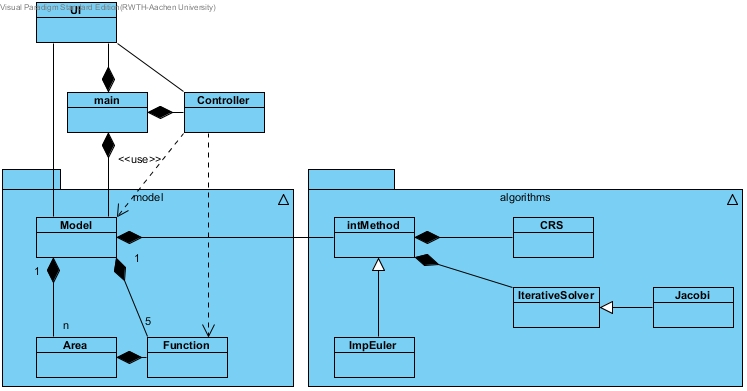
\includegraphics[scale=.62]{Bilder/Paketdiagramm.jpg}\\
	\caption{Paketstruktur}
	\label{Paketdiagramm}
\end{figure}

%\section{Abstrakte Datentypen}
\newpage
\section{Klassen} \label{Kapitel 3 Klassen}

Nachfolgend sind die Klassen-/Sequenzdiagramme nach Paketen sortiert aufgelistet. \\
Dabei werden keine Sequenzdiagramme gezeigt, falls es sich um Methoden ohne Kommunikation mit anderen Objekten handelt, insbesondere keine reinen Getter/Setter-Funktionen oder Funktionen die lediglich Algorithmen implementieren.

\subsection{Paket algorithms}

Das Klassendiagramm in Abbildung \ref{Klassendiagramm algorithms} zeigt alle im Paket \emph{algorithms} enthaltene Klassen und deren Attribute und Funktionen.

%Klassendiagramm algorithms
\begin{figure}[H]
	\centering
	\hspace{-.2cm}
	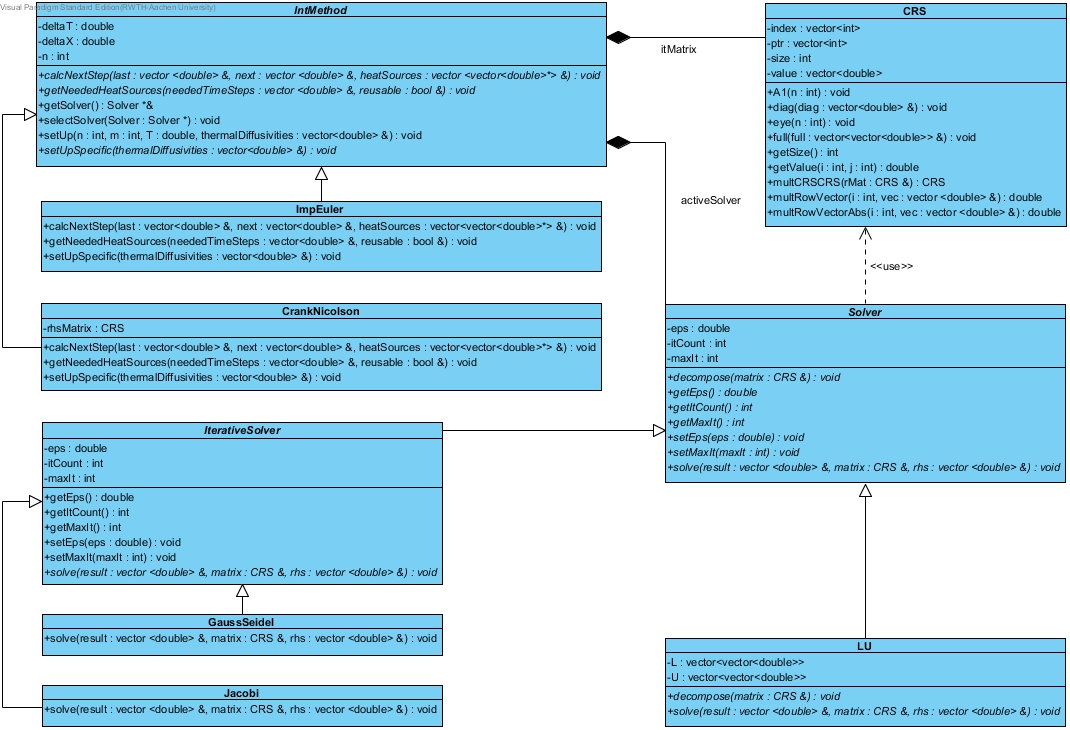
\includegraphics[scale=.49]{Bilder/algorithms.jpg}\\
	\caption{Klassendiagramm algorithms}
	\label{Klassendiagramm algorithms}
\end{figure}
\newpage
\subsubsection{IntMethod}

\subsubsection*{calcNextStep}

Das Sequenzdiagramm für \emph{calcNextStep} ist in Abbildung \ref{Sequenzdiagramm IntMethod::calcNextStep} dargestellt. \emph{calcNextStep} berechnet die Approximation der Temperaturverteilung zum nächsten Zeitpunkt unter Verwendung der aktuellen Verteilung sowie der eingegebenen Temperaturleitkoeffizienten und Wärmequellen.

%Sequenzdiagramm calcNextStep
\begin{figure}[H]
	\centering
	%\hspace{-.5cm}
	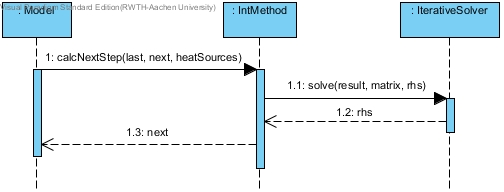
\includegraphics[scale=.7]{Bilder/IntMethod__calcNextStep().jpg}\\
	\caption{Sequenzdiagramm IntMethod::calcNextStep}
	\label{Sequenzdiagramm IntMethod::calcNextStep}
\end{figure}

\subsubsection*{setUpSpecific}

Das Sequenzdiagramm für \emph{setUpSpecific} ist in Abbildung \ref{Sequenzdiagramm setUpSpecific} dargestellt. \emph{setUpSpecific} trifft für die gewählte Integrationsmethode spezifische Vorbereitungen.

%Sequenzdiagramm setUpSpecific
\begin{figure}[H]
	\centering
	%\hspace{-.5cm}
	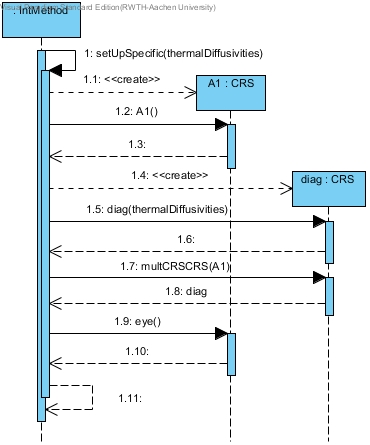
\includegraphics[scale=.6]{Bilder/IntMethod__setUpSpecific().jpg}\\
	\caption{Sequenzdiagramm setUpSpecific}
	\label{Sequenzdiagramm setUpSpecific}
\end{figure}

\newpage
\subsection{Paket model}

Das Klassendiagramm in Abbildung \ref{Klassendiagramm Model} zeigt alle im Paket \emph{model} enthaltene Klassen und deren Attribute und Funktionen.

%Klassendiagramm model
\begin{figure}[H]
	\centering
	%\hspace{-.5cm}
	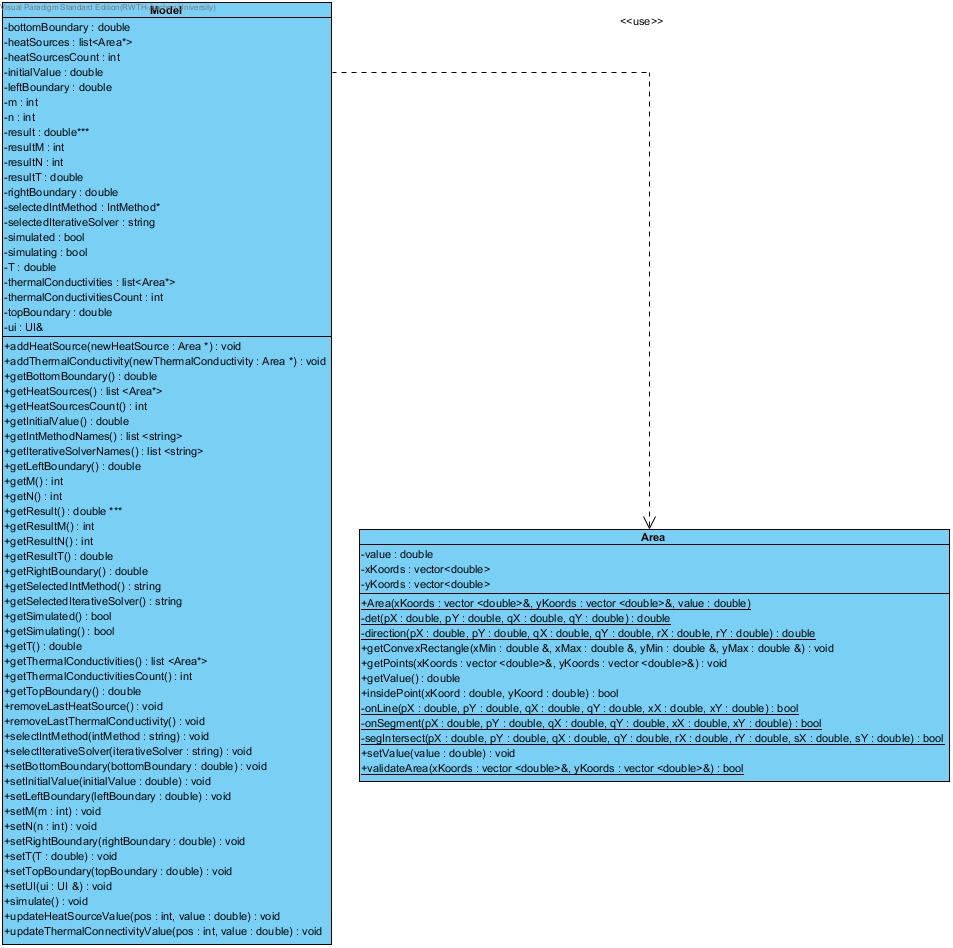
\includegraphics[scale=.36]{Bilder/model.jpg}\\
	\caption{Klassendiagramm Model}
	\label{Klassendiagramm Model}
\end{figure}

\subsubsection{Model}

\subsubsection*{abortWork}

Das Sequenzdiagramm für \emph{abortWork} ist in Abbildung \ref{Sequenzdiagramm Model::abortWork} dargestellt. \emph{abortWork} bricht eine laufende Simulation oder Optimierung ab.

%Sequenzdiagramm abortWork
\begin{figure}[H]
	\centering
	%\hspace{-.5cm}
	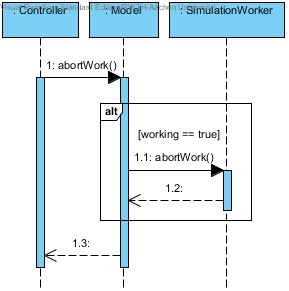
\includegraphics[scale=.85]{Bilder/Model__abortWork().jpg}\\
	\caption{Sequenzdiagramm Model::abortWork}
	\label{Sequenzdiagramm Model::abortWork}
\end{figure}

\subsubsection*{addNewArea}

Das Sequenzdiagramm für \emph{addNewArea} ist in Abbildung \ref{Sequenzdiagramm Model::addNewArea} dargestellt. \emph{addNewArea} fügt ein neues Gebiet vom übergebenen Typ hinzu.

%Sequenzdiagramm addNewArea
\begin{figure}[H]
	\centering
	%\hspace{-.5cm}
	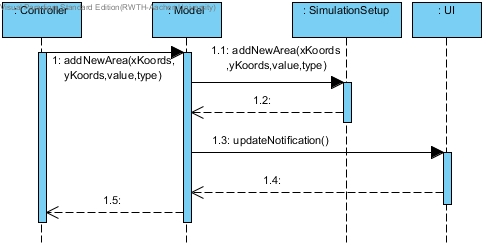
\includegraphics[scale=.85]{Bilder/Model__addNewArea().jpg}\\
	\caption{Sequenzdiagramm Model::addNewArea}
	\label{Sequenzdiagramm Model::addNewArea}
\end{figure}

\subsubsection*{deleteArea}

Das Sequenzdiagramm für \emph{deleteArea} ist in Abbildung \ref{Sequenzdiagramm Model::deleteArea} dargestellt. \emph{deleteArea} löscht das Gebiet vom übergebenen Typ an der übergebenen Position.

%Sequenzdiagramm deleteArea
\begin{figure}[H]
	\centering
	%\hspace{-.5cm}
	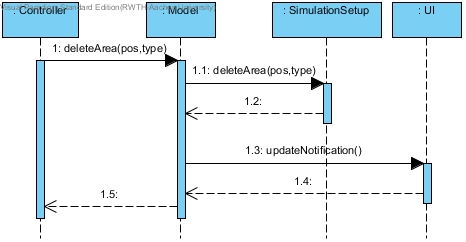
\includegraphics[scale=.85]{Bilder/Model__deleteArea().jpg}\\
	\caption{Sequenzdiagramm Model::deleteArea}
	\label{Sequenzdiagramm Model::deleteArea}
\end{figure}

\subsubsection*{finishedOptimizationSlot}

Das Sequenzdiagramm für \emph{finishedOptimizationSlot} ist in Abbildung \ref{Sequenzdiagramm Model::finishedOptimizationSlot} dargestellt. \emph{finishedOptimizationSlot} informiert das UI über das Ende einer Optimierung.

%Sequenzdiagramm finishedOptimizationSlot
\begin{figure}[H]
	\centering
	%\hspace{-.5cm}
	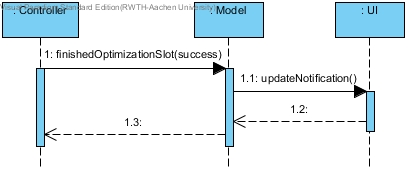
\includegraphics[scale=.85]{Bilder/Model__finishedOptimizationSlot().jpg}\\
	\caption{Sequenzdiagramm Model::finishedOptimizationSlot}
	\label{Sequenzdiagramm Model::finishedOptimizationSlot}
\end{figure}

\subsubsection*{finishedReadingDataSlot}

Das Sequenzdiagramm für \emph{finishedReadingDataSlot} ist in Abbildung \ref{Sequenzdiagramm Model::finishedReadingDataSlot} dargestellt. \emph{finishedReadingDataSlot} informiert das UI über das Ende des Einlesen von Messdaten.

%Sequenzdiagramm finishedReadingDataSlot
\begin{figure}[H]
	\centering
	%\hspace{-.5cm}
	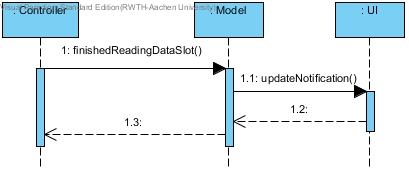
\includegraphics[scale=.85]{Bilder/Model__finishedReadingDataSlot().jpg}
	\caption{Sequenzdiagramm Model::finishedReadingDataSlot}
	\label{Sequenzdiagramm Model::finishedReadingDataSlot}
\end{figure}

\subsubsection*{finishedSimulationSlot}

Das Sequenzdiagramm für \emph{finishedSimulationSlot} ist in Abbildung \ref{Sequenzdiagramm Model::finishedSimulationSlot} dargestellt. \emph{finishedSimulationSlot} informiert das UI über das Ende einer Simulation.

%Sequenzdiagramm finishedSimulationSlot
\begin{figure}[H]
	\centering
	%\hspace{-.5cm}
	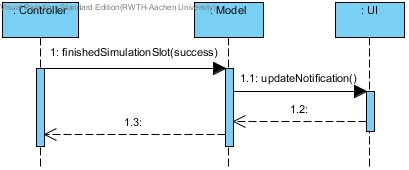
\includegraphics[scale=.85]{Bilder/Model__finishedSimulationSlot().jpg}\\
	\caption{Sequenzdiagramm Model::finishedSimulationSlot}
	\label{Sequenzdiagramm Model::finishedSimulationSlot}
\end{figure}

\subsubsection*{getObservations}

Das Sequenzdiagramm für \emph{getObservations} ist in Abbildung \ref{Sequenzdiagramm Model::getObservations} dargestellt. \emph{getObservations} gibt eingelesene Messdaten zurück, falls bereits welche eingelesen wurden und gerade keine Simulation/Optimierung durchgeführt wird.

%Sequenzdiagramm getObservations
\begin{figure}[H]
	\centering
	%\hspace{-.5cm}
	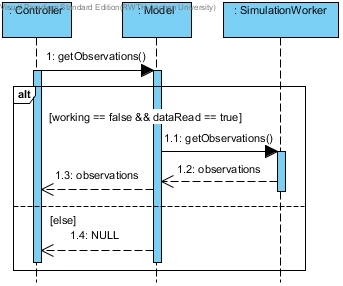
\includegraphics[scale=.85]{Bilder/Model__getObservations().jpg}\\
	\caption{Sequenzdiagramm Model::getObservations}
	\label{Sequenzdiagramm Model::getObservations}
\end{figure}

\subsubsection*{getResult}

Das Sequenzdiagramm für \emph{getResult} ist in Abbildung \ref{Sequenzdiagramm Model::getResult} dargestellt. \emph{getResult} gibt das Ergebnis einer Simulation zurück, falls bereits eine durchgeführt wurde und gerade keine Simulation/Optimierung durchgeführt wird.

%Sequenzdiagramm getResult
\begin{figure}[H]
	\centering
	%\hspace{-.5cm}
	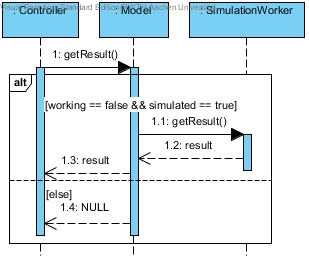
\includegraphics[scale=.85]{Bilder/Model__getResult().jpg}\\
	\caption{Sequenzdiagramm Model::getResult}
	\label{Sequenzdiagramm Model::getResult}
\end{figure}

\subsubsection*{getResultM}

Das Sequenzdiagramm für \emph{getResultM} ist in Abbildung \ref{Sequenzdiagramm Model::getResultM} dargestellt. \emph{getResult} gibt die Zeitdiskretisierungsgröße der letzten Simulation zurück, falls bereits eine durchgeführt wurde und gerade keine Simulation/Optimierung durchgeführt wird.

%Sequenzdiagramm getResultM
\begin{figure}[H]
	\centering
	%\hspace{-.5cm}
	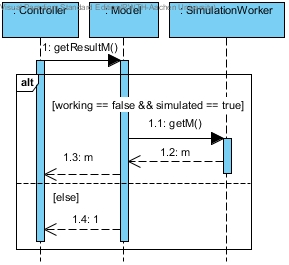
\includegraphics[scale=.85]{Bilder/Model__getResultM().jpg}\\
	\caption{Sequenzdiagramm Model::getResultM}
	\label{Sequenzdiagramm Model::getResultM}
\end{figure}

\subsubsection*{getResultN}

Das Sequenzdiagramm für \emph{getResultN} ist in Abbildung \ref{Sequenzdiagramm Model::getResultN} dargestellt. \emph{getResultN} gibt die Ortsdiskretisierungsgröße der letzten Simulation zurück, falls bereits eine durchgeführt wurde und gerade keine Simulation/Optimierung durchgeführt wird.

%Sequenzdiagramm getResultN
\begin{figure}[H]
	\centering
	%\hspace{-.5cm}
	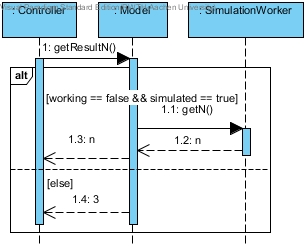
\includegraphics[scale=.85]{Bilder/Model__getResultN().jpg}\\
	\caption{Sequenzdiagramm Model::getResultN}
	\label{Sequenzdiagramm Model::getResultN}
\end{figure}

\subsubsection*{getResultT}

Das Sequenzdiagramm für \emph{getResultT} ist in Abbildung \ref{Sequenzdiagramm Model::getResultT} dargestellt. \emph{getResultT} gibt den Endzeitpunkt der letzten Simulation zurück, falls bereits eine durchgeführt wurde und gerade keine Simulation/Optimierung durchgeführt wird.

%Sequenzdiagramm getResultT
\begin{figure}[H]
	\centering
	%\hspace{-.5cm}
	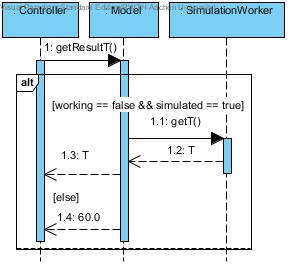
\includegraphics[scale=.85]{Bilder/Model__getResultT().jpg}\\
	\caption{Sequenzdiagramm Model::getResultT}
	\label{Sequenzdiagramm Model::getResultT}
\end{figure}

\subsubsection*{loadSetup}

Das Sequenzdiagramm für \emph{loadSetup} ist in Abbildung \ref{Sequenzdiagramm Model::loadSetup} dargestellt. \emph{loadSetup} lädt gespeicherte Simulationseinstellungen aus einer Datei ein.

%Sequenzdiagramm loadSetup
\begin{figure}[H]
	\centering
	%\hspace{-.5cm}
	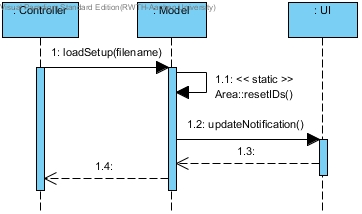
\includegraphics[scale=.85]{Bilder/Model__loadSetup().jpg}\\
	\caption{Sequenzdiagramm Model::loadSetup}
	\label{Sequenzdiagramm Model::loadSetup}
\end{figure}

\subsubsection*{optimize}

Das Sequenzdiagramm für \emph{optimize} ist in Abbildung \ref{Sequenzdiagramm Model::optimize} dargestellt. \emph{optimize} startet eine Optimierung der Temperaturleitkoeffizienten.

%Sequenzdiagramm optimize
\begin{figure}[H]
	\centering
	%\hspace{-.5cm}
	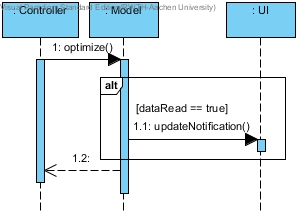
\includegraphics[scale=.85]{Bilder/Model__optimize().jpg}\\
	\caption{Sequenzdiagramm Model::optimize}
	\label{Sequenzdiagramm Model::optimize}
\end{figure}

\subsubsection*{readObservations}

Das Sequenzdiagramm für \emph{readObservations} ist in Abbildung \ref{Sequenzdiagramm Model::readObservations} dargestellt. \emph{readObservations} startet das Einlesen von Messdaten für eine Optimierung.

%Sequenzdiagramm readObservations
\begin{figure}[H]
	\centering
	%\hspace{-.5cm}
	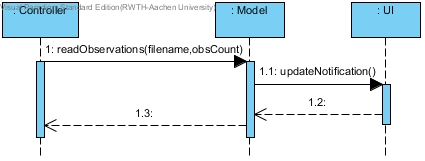
\includegraphics[scale=.85]{Bilder/Model__readObservations().jpg}\\
	\caption{Sequenzdiagramm Model::readObservations}
	\label{Sequenzdiagramm Model::readObservations}
\end{figure}

\subsubsection*{removeLastArea}

Das Sequenzdiagramm für \emph{removeLastArea} ist in Abbildung \ref{Sequenzdiagramm Model::removeLastArea} dargestellt. \emph{removeLastArea} entfernt das letzte hinzugefügte Gebiet vom übergebenen Typ.

%Sequenzdiagramm removeLastArea
\begin{figure}[H]
	\centering
	%\hspace{-.5cm}
	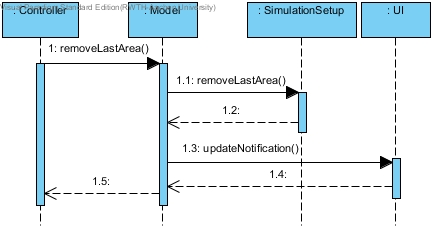
\includegraphics[scale=.85]{Bilder/Model__removeLastArea().jpg}\\
	\caption{Sequenzdiagramm Model::removeLastArea}
	\label{Sequenzdiagramm Model::removeLastArea}
\end{figure}

\subsubsection*{reorderArea}

Das Sequenzdiagramm für \emph{reorderArea} ist in Abbildung \ref{Sequenzdiagramm Model::reorderArea} dargestellt. \emph{reorderArea} ändert die Reihenfolge der Gebiete vom übergebenen Typ.

%Sequenzdiagramm reorderArea
\begin{figure}[H]
	\centering
	%\hspace{-.5cm}
	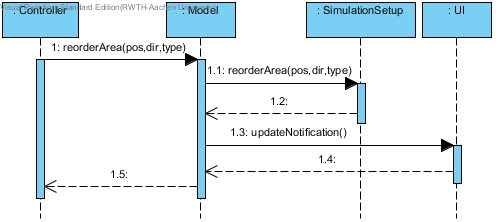
\includegraphics[scale=.85]{Bilder/Model__reorderArea().jpg}\\
	\caption{Sequenzdiagramm Model::reorderArea}
	\label{Sequenzdiagramm Model::reorderArea}
\end{figure}

\subsubsection*{resetSetup}

Das Sequenzdiagramm für \emph{resetSetup} ist in Abbildung \ref{Sequenzdiagramm Model::resetSetup} dargestellt. \emph{resetSetup} setzt die Simulationseinstellungen auf die Standardwerte zurück.

%Sequenzdiagramm resetSetup
\begin{figure}[H]
	\centering
	%\hspace{-.5cm}
	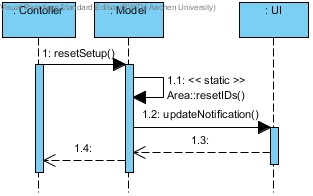
\includegraphics[scale=.85]{Bilder/Model__resetSetup().jpg}\\
	\caption{Sequenzdiagramm Model::resetSetup}
	\label{Sequenzdiagramm Model::resetSetup}
\end{figure}

\subsubsection*{selectIntMethod}

Das Sequenzdiagramm für \emph{selectIntMethod} ist in Abbildung \ref{Sequenzdiagramm Model::selectIntMethod} dargestellt. \emph{selectIntMethod} setzt die Integrationsmethode für die Simulation.

%Sequenzdiagramm selectIntMethod
\begin{figure}[H]
	\centering
	%\hspace{-.5cm}
	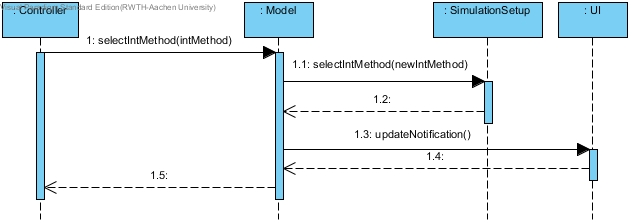
\includegraphics[scale=.8]{Bilder/Model__selectIntMethod().jpg}\\
	\caption{Sequenzdiagramm Model::selectIntMethod}
	\label{Sequenzdiagramm Model::selectIntMethod}
\end{figure}

\subsubsection*{selectSolver}

Das Sequenzdiagramm für \emph{selectSolver} ist in Abbildung \ref{Sequenzdiagramm Model::selectSolver} dargestellt. \emph{selectSolver} setzt den LGS Löser für die Simulation.

%Sequenzdiagramm selectSolver
\begin{figure}[H]
	\centering
	%\hspace{-.5cm}
	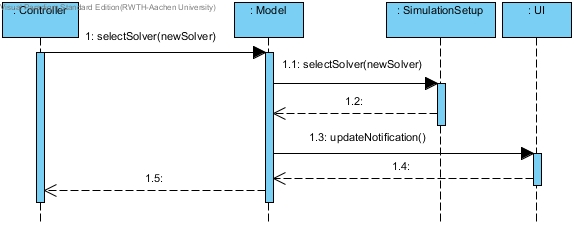
\includegraphics[scale=.8]{Bilder/Model__selectSolver().jpg}\\
	\caption{Sequenzdiagramm Model::selectSolver}
	\label{Sequenzdiagramm Model::selectSolver}
\end{figure}

\subsubsection*{setAreaBackgroundValue}

Das Sequenzdiagramm für \emph{setAreaBackgroundValue} ist in Abbildung \ref{Sequenzdiagramm Model::setAreaBackgroundValue} dargestellt. \emph{setAreaBackgroundValue} setzt den Hintergrundwert für die Gebiete des übergebenen Typs.

%Sequenzdiagramm setAreaBackgroundValue
\begin{figure}[H]
	\centering
	%\hspace{-.5cm}
	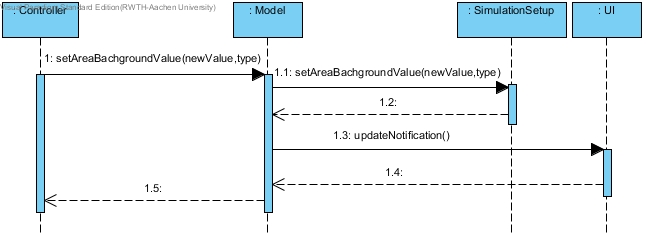
\includegraphics[scale=.8]{Bilder/Model__setAreaBackgroundValue().jpg}\\
	\caption{Sequenzdiagramm Model::setAreaBackgroundValue}
	\label{Sequenzdiagramm Model::setAreaBackgroundValue}
\end{figure}

\subsubsection*{setIBV}

Das Sequenzdiagramm für \emph{setIBV} ist in Abbildung \ref{Sequenzdiagramm Model::setIBV} dargestellt. \emph{setIBV} setzt einen der Randwerte oder den Anfangswert für die Simulation.

%Sequenzdiagramm setIBV
\begin{figure}[H]
	\centering
	%\hspace{-.5cm}
	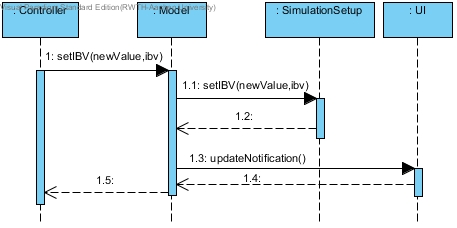
\includegraphics[scale=.85]{Bilder/Model__setIBV().jpg}\\
	\caption{Sequenzdiagramm Model::setIBV}
	\label{Sequenzdiagramm Model::setIBV}
\end{figure}

\subsubsection*{setM}

Das Sequenzdiagramm für \emph{setM} ist in Abbildung \ref{Sequenzdiagramm Model::setM} dargestellt. \emph{setM} setzt die Zeitdiskretisierungsgröße für die Simulation.

%Sequenzdiagramm setM
\begin{figure}[H]
	\centering
	%\hspace{-.5cm}
	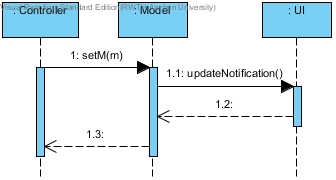
\includegraphics[scale=.85]{Bilder/Model__setM().jpg}\\
	\caption{Sequenzdiagramm Model::setM}
	\label{Sequenzdiagramm Model::setM}
\end{figure}

\subsubsection*{setN}

Das Sequenzdiagramm für \emph{setN} ist in Abbildung \ref{Sequenzdiagramm Model::setN} dargestellt. \emph{setN} setzt die Ortsdiskretisierungsgröße für die Simulation.

%Sequenzdiagramm setN
\begin{figure}[H]
	\centering
	%\hspace{-.5cm}
	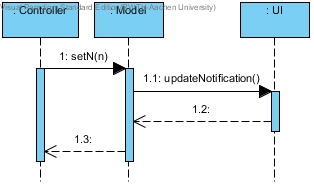
\includegraphics[scale=.85]{Bilder/Model__setN().jpg}\\
	\caption{Sequenzdiagramm Model::setN}
	\label{Sequenzdiagramm Model::setN}
\end{figure}

\subsubsection*{setOverrideThermalDiffusivities}

Das Sequenzdiagramm für \emph{setOverrideThermalDiffusivities} ist in Abbildung \ref{Sequenzdiagramm Model::setOverrideThermalDiffusivities} dargestellt. \emph{setOverrideThermalDiffusivities} aktiviert die Nutzung des manuellen Anfangswertes für die Optimierung.

%Sequenzdiagramm setOverrideThermalDiffusivities
\begin{figure}[H]
	\centering
	%\hspace{-.5cm}
	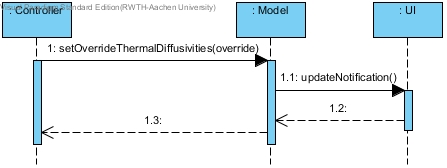
\includegraphics[scale=.85]{Bilder/Model__setOverrideThermalDiffusivities().jpg}\\
	\caption{Sequenzdiagramm Model::setOverrideThermalDiffusivities}
	\label{Sequenzdiagramm Model::setOverrideThermalDiffusivities}
\end{figure}

\subsubsection*{setOverrideValue}

Das Sequenzdiagramm für \emph{setOverrideValue} ist in Abbildung \ref{Sequenzdiagramm Model::setOverrideValue} dargestellt. \emph{setOverrideValue} setzt den manuellen Anfangswert für die Optimierung.

%Sequenzdiagramm setOverrideValue
\begin{figure}[H]
	\centering
	%\hspace{-.5cm}
	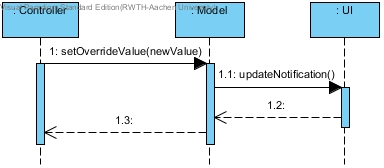
\includegraphics[scale=.85]{Bilder/Model__setOverrideValue().jpg}\\
	\caption{Sequenzdiagramm Model::setOverrideValue}
	\label{Sequenzdiagramm Model::setOverrideValue}
\end{figure}

\subsubsection*{setSolverMaxError}

Das Sequenzdiagramm für \emph{setSolverMaxError} ist in Abbildung \ref{Sequenzdiagramm Model::setSolverMaxError} dargestellt. \emph{setSolverMaxError} setzt die relative Fehlertoleranz des LGS Lösers.

%Sequenzdiagramm setSolverMaxError
\begin{figure}[H]
	\centering
	%\hspace{-.5cm}
	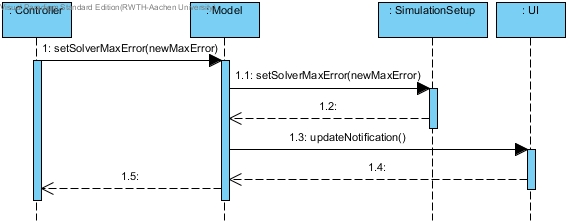
\includegraphics[scale=.85]{Bilder/Model__setSolverMaxError().jpg}\\
	\caption{Sequenzdiagramm Model::setSolverMaxError}
	\label{Sequenzdiagramm Model::setSolverMaxError}
\end{figure}

\subsubsection*{setSolverMaxIt}

Das Sequenzdiagramm für \emph{setSolverMaxIt} ist in Abbildung \ref{Sequenzdiagramm Model::setSolverMaxIt} dargestellt. \emph{setSolverMaxIt} setzt die maximale Iterationsanzahl des LGS Lösers.

%Sequenzdiagramm setSolverMaxIt
\begin{figure}[H]
	\centering
	%\hspace{-.5cm}
	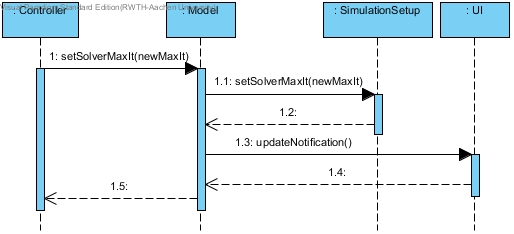
\includegraphics[scale=.85]{Bilder/Model__setSolverMaxIt().jpg}\\
	\caption{Sequenzdiagramm Model::setSolverMaxIt}
	\label{Sequenzdiagramm Model::setSolverMaxIt}
\end{figure}

\subsubsection*{setT}

Das Sequenzdiagramm für \emph{setT} ist in Abbildung \ref{Sequenzdiagramm Model::setT} dargestellt. \emph{setT} setzt den Endzeitpunkt für die Simulation.

%Sequenzdiagramm setT
\begin{figure}[H]
	\centering
	%\hspace{-.5cm}
	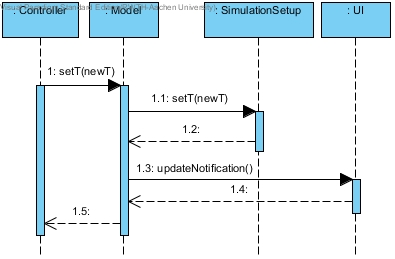
\includegraphics[scale=.85]{Bilder/Model__setT().jpg}\\
	\caption{Sequenzdiagramm Model::setT}
	\label{Sequenzdiagramm Model::setT}
\end{figure}

\subsubsection*{setUseHeatSources}

Das Sequenzdiagramm für \emph{setUseHeatSources} ist in Abbildung \ref{Sequenzdiagramm Model::setUseHeatSources} dargestellt. \emph{setUseHeatSources} aktiviert die Nutzung der Wärmequellen-Gebiete für die Optimierung.

%Sequenzdiagramm setUseHeatSources
\begin{figure}[H]
	\centering
	%\hspace{-.5cm}
	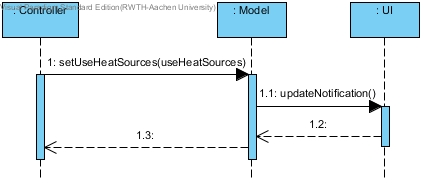
\includegraphics[scale=.85]{Bilder/Model__setUseHeatSources().jpg}\\
	\caption{Sequenzdiagramm Model::setUseHeatSources}
	\label{Sequenzdiagramm Model::setUseHeatSources}
\end{figure}

\subsubsection*{simulate}

Das Sequenzdiagramm für \emph{simulate} ist in Abbildung \ref{Sequenzdiagramm Model::simulate} dargestellt. \emph{simulate} startet eine Simulation der Wärmeleitungsgleichung.

%Sequenzdiagramm simulate
\begin{figure}[H]
	\centering
	%\hspace{-.5cm}
	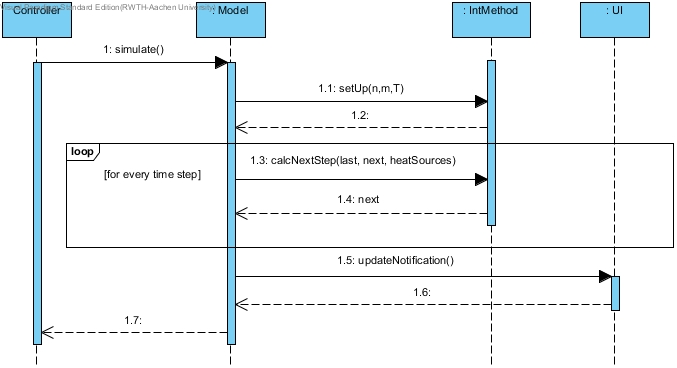
\includegraphics[scale=.85]{Bilder/Model__simulate().jpg}\\
	\caption{Sequenzdiagramm Model::simulate}
	\label{Sequenzdiagramm Model::simulate}
\end{figure}

\subsubsection*{updateAreaValue}

Das Sequenzdiagramm für \emph{updateAreaValue} ist in Abbildung \ref{Sequenzdiagramm Model::updateAreaValue} dargestellt. \emph{updateAreaValue} ändert den Wert eines Gebietes vom übergebenen Typ.

%Sequenzdiagramm updateAreaValue
\begin{figure}[H]
	\centering
	%\hspace{-.5cm}
	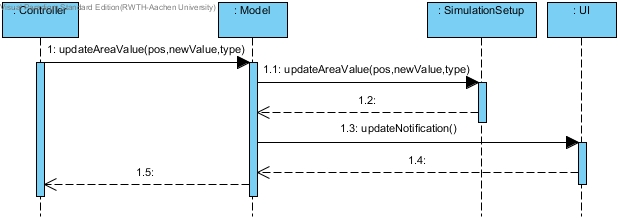
\includegraphics[scale=.8]{Bilder/Model__updateAreaValue().jpg}\\
	\caption{Sequenzdiagramm Model::updateAreaValue}
	\label{Sequenzdiagramm Model::updateAreaValue}
\end{figure}

\newpage
\subsubsection{SimulationSetup}

\subsubsection*{getContainingAreaID}

Das Sequenzdiagramm für \emph{getContainingAreaID} ist in Abbildung \ref{Sequenzdiagramm SimulationSetup::getContainingAreaID} dargestellt. \emph{getContainingAreaID} findet die ID des ersten Gebietes, das den übergebenen Punkt enthält.

%Sequenzdiagramm getContainingAreaID
\begin{figure}[H]
	\centering
	%\hspace{-.5cm}
	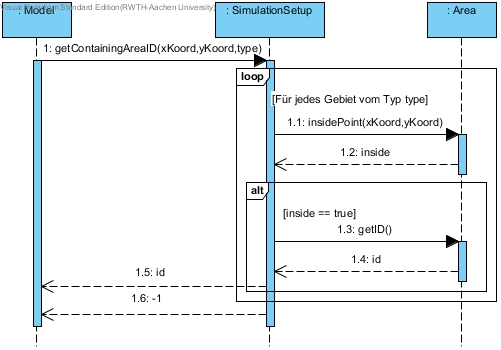
\includegraphics[scale=1]{Bilder/SimulationSetup__getContainingAreaID().jpg}\\
	\caption{Sequenzdiagramm SimulationSetup::getContainingAreaID}
	\label{Sequenzdiagramm SimulationSetup::getContainingAreaID}
\end{figure}

\subsubsection*{updateAreaValue}

Das Sequenzdiagramm für \emph{updateAreaValue} ist in Abbildung \ref{Sequenzdiagramm SimulationSetup::updateAreaValue} dargestellt. \emph{updateAreaValue} ändert den Wert des Gebietes vom übergebenen Typ an der übergebenen Position.

%Sequenzdiagramm updateAreaValue
\begin{figure}[H]
	\centering
	%\hspace{-.5cm}
	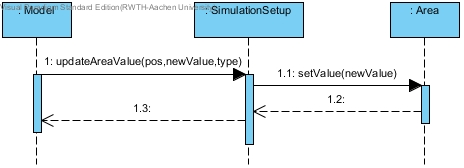
\includegraphics[scale=1]{Bilder/SimulationSetup__updateAreaValue().jpg}\\
	\caption{Sequenzdiagramm SimulationSetup::updateAreaValue}
	\label{Sequenzdiagramm SimulationSetup::updateAreaValue}
\end{figure}

\subsubsection{SimulationWorker}

\subsubsection*{simpleSimulation}

Das Sequenzdiagramm für \emph{simpleSimulation} ist in Abbildung \ref{Sequenzdiagramm SimulationWorker::simpleSimulation} dargestellt. \emph{simpleSimulation} führt eine Simulation der Wärmeleitungsgleichung ohne Speichern der Zwischenschritte (für die Optimierung).

%Sequenzdiagramm simpleSimulation
\begin{figure}[H]
	\centering
	%\hspace{-.5cm}
	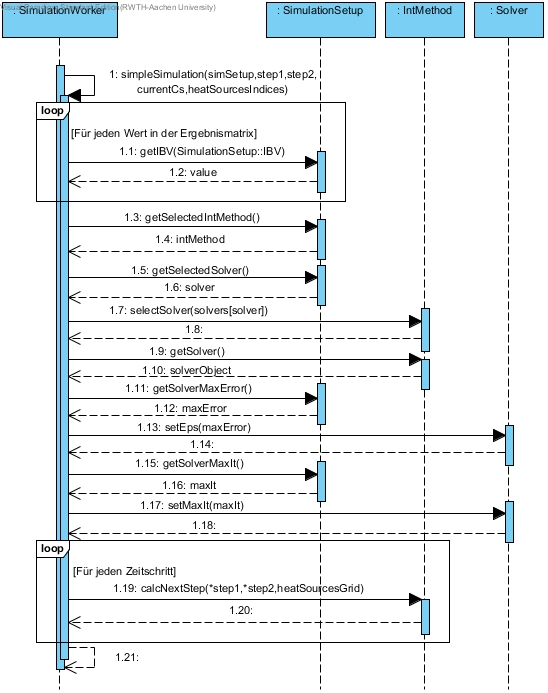
\includegraphics[scale=.85]{Bilder/SimulationWorker__simpleSimulation().jpg}\\
	\caption{Sequenzdiagramm SimulationWorker::simpleSimulation}
	\label{Sequenzdiagramm SimulationWorker::simpleSimulation}
\end{figure}

\subsubsection*{startOptimizationSlot}

Das Sequenzdiagramm für \emph{startOptimizationSlot} ist in Abbildung \ref{Sequenzdiagramm SimulationWorker::startOptimizationSlot} dargestellt. \emph{startOptimizationSlot} führt eine Optimierung der Temperaturleitkoeffizienten durch.

%Sequenzdiagramm startOptimizationSlot
\begin{figure}[H]
	\centering
	%\hspace{-.5cm}
	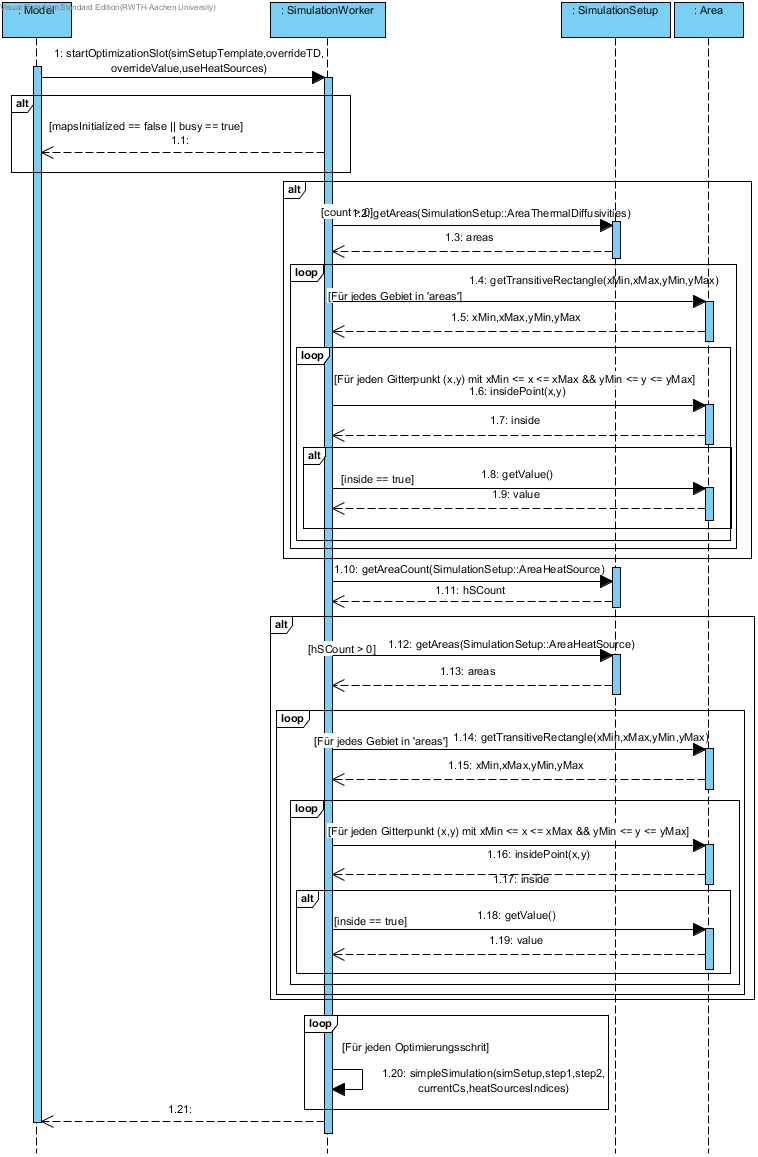
\includegraphics[scale=.55]{Bilder/SimulationWorker__startOptimizationSlot().jpg}\\
	\caption{Sequenzdiagramm SimulationWorker::startOptimizationSlot}
	\label{Sequenzdiagramm SimulationWorker::startOptimizationSlot}
\end{figure}

\subsubsection*{startSimulationSlot}

Das Sequenzdiagramm für \emph{startSimulationSlot} ist in Abbildung \ref{Sequenzdiagramm SimulationWorker::startSimulationSlot} dargestellt. \emph{startSimulationSlot} führt eine Simulation der Wärmleitungsgleichung durch.

%Sequenzdiagramm startSimulationSlot
\begin{figure}[H]
	\centering
	%\hspace{-.5cm}
	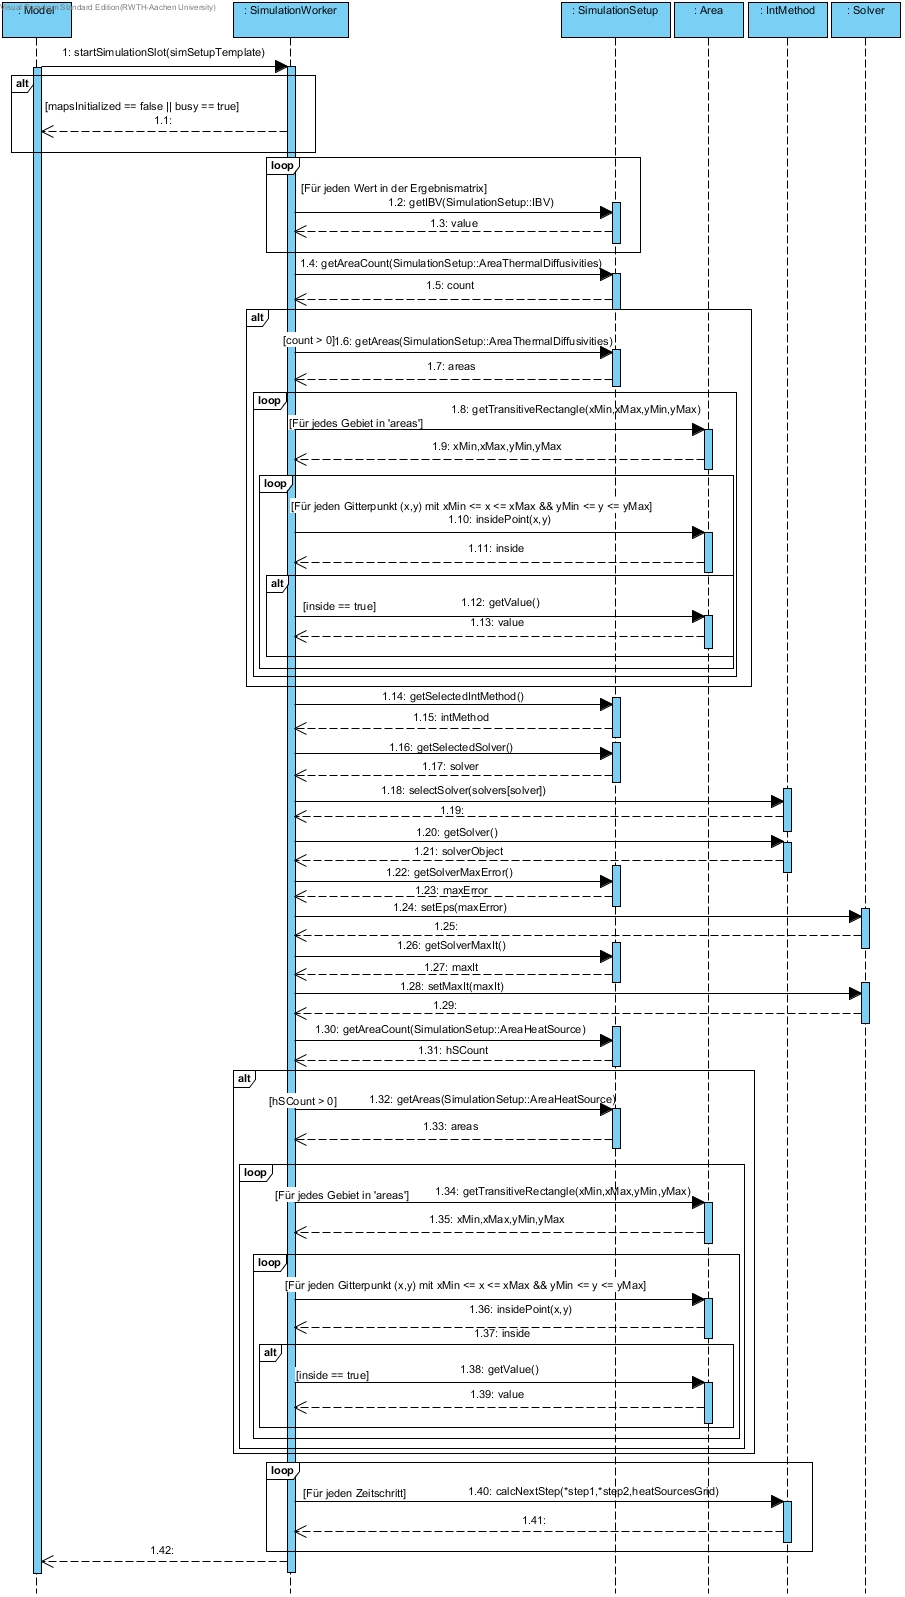
\includegraphics[scale=.4]{Bilder/SimulationWorker__startSimulationSlot().jpg}\\
	\caption{Sequenzdiagramm SimulationWorker::startSimulationSlot}
	\label{Sequenzdiagramm SimulationWorker::startSimulationSlot}
\end{figure}

\newpage
\subsection{Paket presentation}

Das Klassendiagramm in Abbildung \ref{Klassendiagramm presentation} zeigt alle im Paket \emph{presentation} enthaltene Klassen.

%Klassendiagramm presentation
\begin{figure}[H]
	\centering
	%\hspace{-.5cm}
	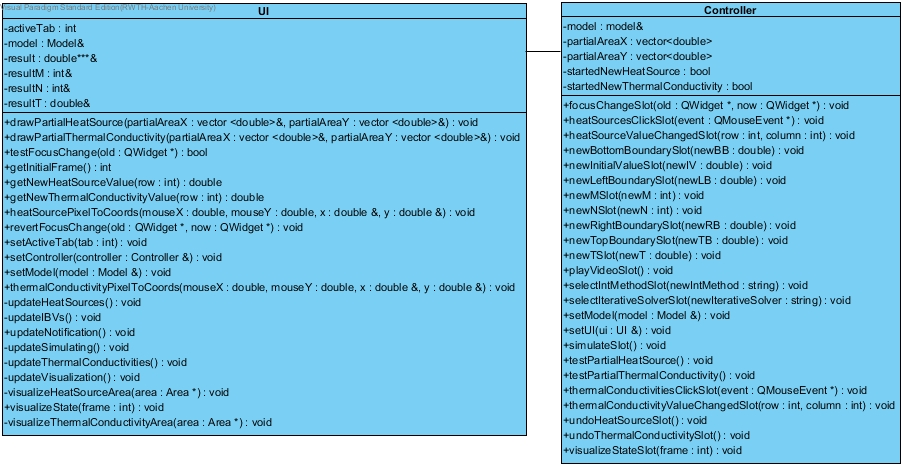
\includegraphics[scale=.42]{Bilder/presentation.jpg}\\
	\caption{Klassendiagramm presentation}
	\label{Klassendiagramm presentation}
\end{figure}

\subsubsection{AreaWidget}

\subsubsection*{drawPartialArea}

Das Sequenzdiagramm für \emph{drawPartialArea} ist in Abbildung \ref{Sequenzdiagramm AreaWidget::drawPartialArea} dargestellt. \emph{drawPartialArea} zeichnet ein neues angefangenes Gebiet.

%Sequenzdiagramm drawPartialArea
\begin{figure}[H]
	\centering
	%\hspace{-.5cm}
	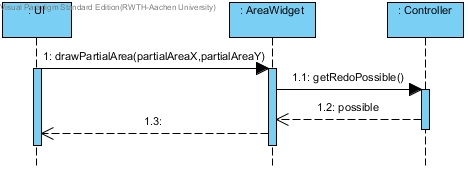
\includegraphics[scale=.85]{Bilder/AreaWidget__drawPartialArea().jpg}\\
	\caption{Sequenzdiagramm AreaWidget::drawPartialArea}
	\label{Sequenzdiagramm AreaWidget::drawPartialArea}
\end{figure}

\subsubsection*{update}

Das Sequenzdiagramm für \emph{update} ist in Abbildung \ref{Sequenzdiagramm AreaWidget::update} dargestellt. \emph{update} aktualisiert den Tab zur Gebietseingabe.

%Sequenzdiagramm update
\begin{figure}[H]
	\centering
	%\hspace{-.5cm}
	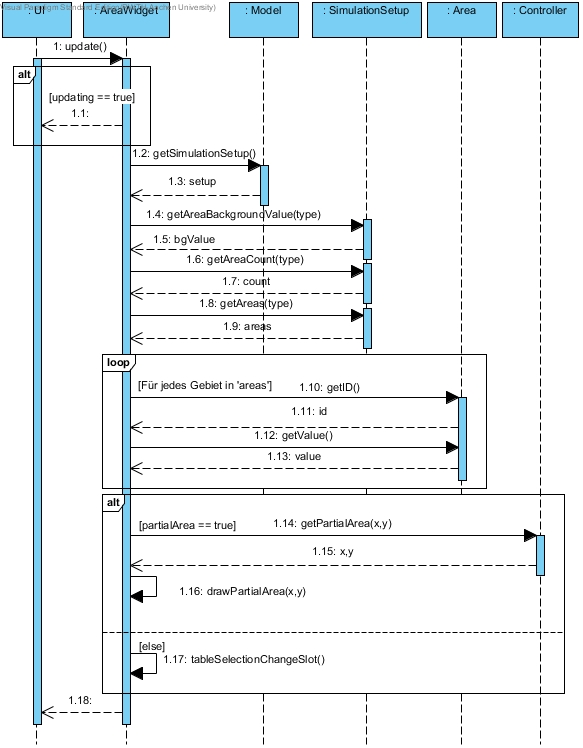
\includegraphics[scale=.85]{Bilder/AreaWidget__update().jpg}\\
	\caption{Sequenzdiagramm AreaWidget::update}
	\label{Sequenzdiagramm AreaWidget::update}
\end{figure}

\subsubsection{Controller}

\subsubsection*{abortWorkSlot}

Das Sequenzdiagramm für \emph{abortWorkSlot} ist in Abbildung \ref{Sequenzdiagramm Controller::abortWorkSlot} dargestellt. \emph{abortWorkSlot} bricht eine laufende Simulation/Optimierung ab.

%Sequenzdiagramm abortWorkSlot
\begin{figure}[H]
	\centering
	%\hspace{-.5cm}
	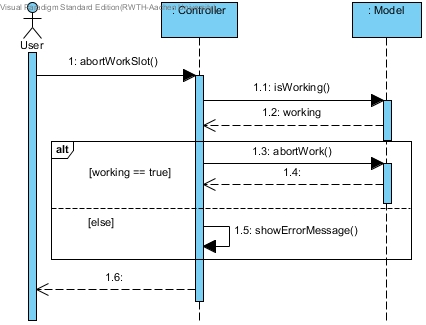
\includegraphics[scale=.6]{Bilder/Controller__abortWorkSlot().jpg}\\
	\caption{Sequenzdiagramm Controller::abortWorkSlot}
	\label{Sequenzdiagramm Controller::abortWorkSlot}
\end{figure}

\subsubsection*{areaClickSlot}

Das Sequenzdiagramm für \emph{areaClickSlot} ist in Abbildung \ref{Sequenzdiagramm Controller::areaClickSlot} dargestellt. \emph{areaClickSlot} verwaltet Mausklicke auf eine der beiden Gebiet-Platten.

%Sequenzdiagramm areaClickSlot
\begin{figure}[H]
	\centering
	%\hspace{-.5cm}
	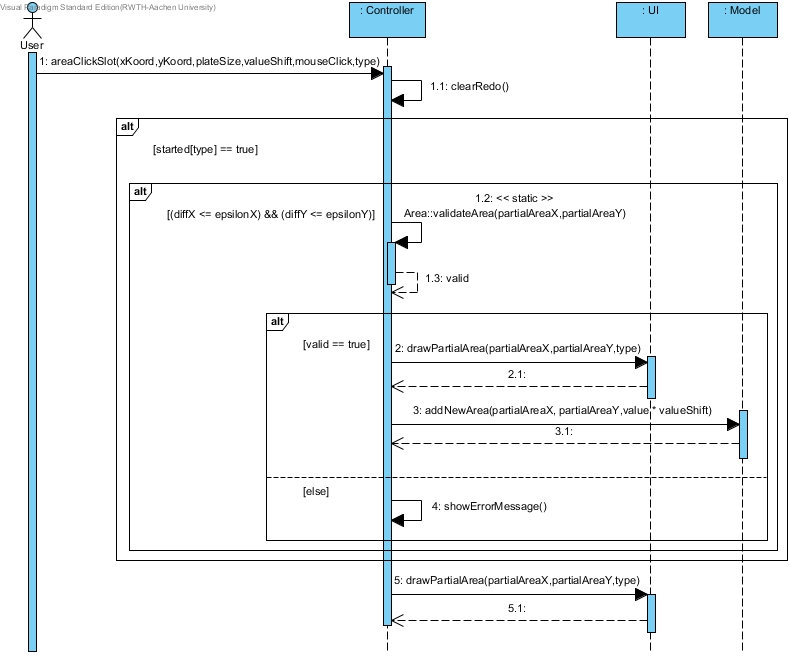
\includegraphics[scale=.5]{Bilder/Controller__areaClickSlot().jpg}\\
	\caption{Sequenzdiagramm Controller::areaClickSlot}
	\label{Sequenzdiagramm Controller::areaClickSlot}
\end{figure}

\subsubsection*{areaValueChangedSlot}

Das Sequenzdiagramm für \emph{areaValueChangedSlot} ist in Abbildung \ref{Sequenzdiagramm Controller::areaValueChangedSlot} dargestellt. \emph{areaValueChangedSlot} verwaltet das Ändern der Werte der verschiedenen Gebiete.

%Sequenzdiagramm areaValueChangedSlot
\begin{figure}[H]
	\centering
	%\hspace{-.5cm}
	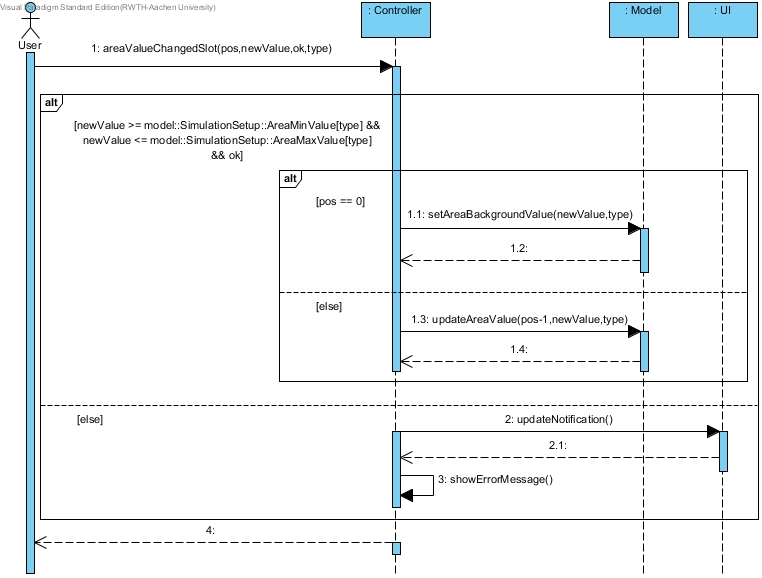
\includegraphics[scale=.5]{Bilder/Controller__areaValueChangedSlot().jpg}\\
	\caption{Sequenzdiagramm Controller::areaValueChangedSlot}
	\label{Sequenzdiagramm Controller::areaValueChangedSlot}
\end{figure}

\subsubsection*{clearAreasSlot}

Das Sequenzdiagramm für \emph{clearAreasSlot} ist in Abbildung \ref{Sequenzdiagramm Controller::clearAreasSlot} dargestellt. \emph{clearAreasSlot} löscht alle Gebiete eines Types.

%Sequenzdiagramm clearAreasSlot
\begin{figure}[H]
	\centering
	%\hspace{-.5cm}
	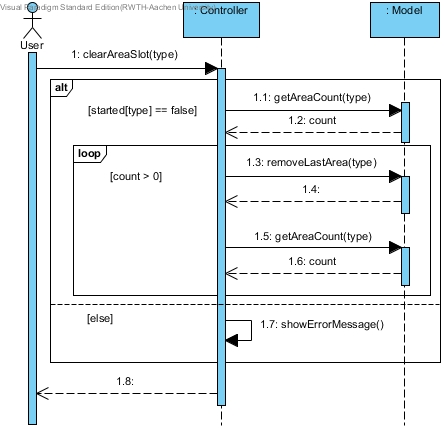
\includegraphics[scale=.6]{Bilder/Controller__clearAreasSlot().jpg}\\
	\caption{Sequenzdiagramm Controller::clearAreasSlot}
	\label{Sequenzdiagramm Controller::clearAreasSlot}
\end{figure}

\subsubsection*{deleteAreaSlot}

Das Sequenzdiagramm für \emph{deleteAreaSlot} ist in Abbildung \ref{Sequenzdiagramm Controller::deleteAreaSlot} dargestellt. \emph{deleteAreaSlot} löscht ein Gebiet eines Types.

%Sequenzdiagramm deleteAreaSlot
\begin{figure}[H]
	\centering
	%\hspace{-.5cm}
	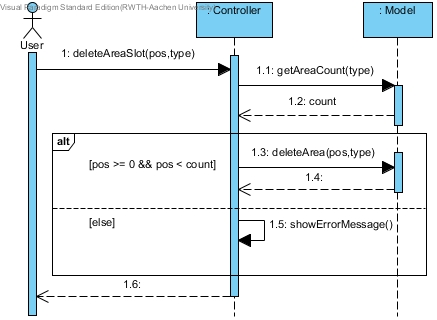
\includegraphics[scale=.85]{Bilder/Controller__deleteAreaSlot().jpg}\\
	\caption{Sequenzdiagramm Controller::deleteAreaSlot}
	\label{Sequenzdiagramm Controller::deleteAreaSlot}
\end{figure}

\subsubsection*{discardAreaSlot}

Das Sequenzdiagramm für \emph{discardAreaSlot} ist in Abbildung \ref{Sequenzdiagramm Controller::discardAreaSlot} dargestellt. \emph{discardAreaSlot} bricht das Erstellen eines neuen Gebietes ab.

%Sequenzdiagramm discardAreaSlot
\begin{figure}[H]
	\centering
	%\hspace{-.5cm}
	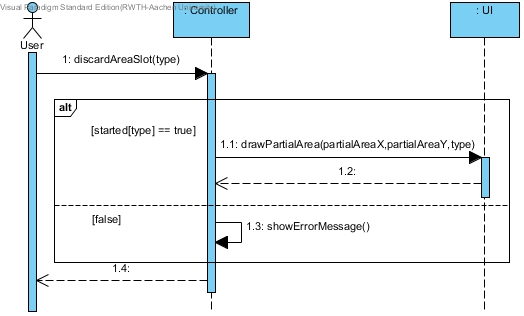
\includegraphics[scale=.85]{Bilder/Controller__discardAreaSlot().jpg}\\
	\caption{Sequenzdiagramm Controller::discardAreaSlot}
	\label{Sequenzdiagramm Controller::discardAreaSlot}
\end{figure}

\subsubsection*{loadObservationsSlot}

Das Sequenzdiagramm für \emph{loadObservationsSlot} ist in Abbildung \ref{Sequenzdiagramm Controller::loadObservationsSlot} dargestellt. \emph{loadObservationsSlot} verwaltet das Einlesen von Messdaten für die Optimierung.

%Sequenzdiagramm loadObservationsSlot
\begin{figure}[H]
	\centering
	%\hspace{-.5cm}
	\includegraphics[scale=.5]{Bilder/Controller__loadObservationsSlot().jpg}\\
	\caption{Sequenzdiagramm Controller::loadObservationsSlot}
	\label{Sequenzdiagramm Controller::loadObservationsSlot}
\end{figure}

\subsubsection*{loadSimulationSetupSlot}

Das Sequenzdiagramm für \emph{loadSimulationSetupSlot} ist in Abbildung \ref{Sequenzdiagramm Controller::loadSimulationSetupSlot} dargestellt. \emph{loadSimulationSetupSlot} verwaltet das Einlesen von gespeicherten Simulationseinstellungen.

%Sequenzdiagramm loadSimulationSetupSlot
\begin{figure}[H]
	\centering
	%\hspace{-.5cm}
	\includegraphics[scale=.6]{Bilder/Controller__loadSimulationSetupSlot().jpg}\\
	\caption{Sequenzdiagramm Controller::loadSimulationSetupSlot}
	\label{Sequenzdiagramm Controller::loadSimulationSetupSlot}
\end{figure}

\subsubsection*{newIBVValueSlot}

Das Sequenzdiagramm für \emph{newIBVValueSlot} ist in Abbildung \ref{Sequenzdiagramm Controller::newIBVValueSlot} dargestellt. \emph{newIBVValueSlot} verwaltet das Ändern eines Rand- bzw. des Anfangswertes.

%Sequenzdiagramm newIBVValueSlot
\begin{figure}[H]
	\centering
	%\hspace{-.5cm}
	\includegraphics[scale=.7]{Bilder/Controller__newIBVValueSlot().jpg}\\
	\caption{Sequenzdiagramm Controller::newIBVValueSlot}
	\label{Sequenzdiagramm Controller::newIBVValueSlot}
\end{figure}

\subsubsection*{newMaxErrorSlot}

Das Sequenzdiagramm für \emph{newMaxErrorSlot} ist in Abbildung \ref{Sequenzdiagramm Controller::newMaxErrorSlot} dargestellt. \emph{newMaxErrorSlot} verwaltet das Ändern der Fehlertoleranz des LGS Lösers.

%Sequenzdiagramm newMaxErrorSlot
\begin{figure}[H]
	\centering
	%\hspace{-.5cm}
	\includegraphics[scale=.7]{Bilder/Controller__newMaxErrorSlot().jpg}\\
	\caption{Sequenzdiagramm Controller::newMaxErrorSlot}
	\label{Sequenzdiagramm Controller::newMaxErrorSlot}
\end{figure}

\subsubsection*{newMaxItSlot}

Das Sequenzdiagramm für \emph{newMaxItSlot} ist in Abbildung \ref{Sequenzdiagramm Controller::newMaxItSlot} dargestellt. \emph{newMaxItSlot} verwaltet das Ändern der maximalen Iterationsanzahl des LGS Lösers.

%Sequenzdiagramm newMaxItSlot
\begin{figure}[H]
	\centering
	%\hspace{-.5cm}
	\includegraphics[scale=.65]{Bilder/Controller__newMaxItSlot().jpg}\\
	\caption{Sequenzdiagramm Controller::newMaxItSlot}
	\label{Sequenzdiagramm Controller::newMaxItSlot}
\end{figure}

\subsubsection*{newMSlot}

Das Sequenzdiagramm für \emph{newMSlot} ist in Abbildung \ref{Sequenzdiagramm Controller::newMSlot} dargestellt. \emph{newMSlot} verwaltet das Ändern der Zeitdiskretisierungsgröße für die Simulation.

%Sequenzdiagramm newMSlot
\begin{figure}[H]
	\centering
	%\hspace{-.5cm}
	\includegraphics[scale=.6]{Bilder/Controller__newMSlot().jpg}\\
	\caption{Sequenzdiagramm Controller::newMSlot}
	\label{Sequenzdiagramm Controller::newMSlot}
\end{figure}

\subsubsection*{newNSlot}

Das Sequenzdiagramm für \emph{newNSlot} ist in Abbildung \ref{Sequenzdiagramm Controller::newNSlot} dargestellt. \emph{newNSlot} verwaltet das Ändern der Ortsdiskretisierungsgröße für die Simulation.

%Sequenzdiagramm newNSlot
\begin{figure}[H]
	\centering
	%\hspace{-.5cm}
	\includegraphics[scale=.55]{Bilder/Controller__newNSlot().jpg}\\
	\caption{Sequenzdiagramm Controller::newNSlot}
	\label{Sequenzdiagramm Controller::newNSlot}
\end{figure}

\subsubsection*{newOverrideValueSlot}

Das Sequenzdiagramm für \emph{newOverrideValueSlot} ist in Abbildung \ref{Sequenzdiagramm Controller::newOverrideValueSlot} dargestellt. \emph{newOverrideValueSlot} verwaltet das Ändern des manuellen Anfangswertes für die Optimierung.

%Sequenzdiagramm newOverrideValueSlot
\begin{figure}[H]
	\centering
	%\hspace{-.5cm}
	\includegraphics[scale=.65]{Bilder/Controller__newOverrideValueSlot().jpg}\\
	\caption{Sequenzdiagramm Controller::newOverrideValueSlot}
	\label{Sequenzdiagramm Controller::newOverrideValueSlot}
\end{figure}

\subsubsection*{newTSlot}

Das Sequenzdiagramm für \emph{newTSlot} ist in Abbildung \ref{Sequenzdiagramm Controller::newTSlot} dargestellt. \emph{newTSlot} verwaltet das Ändern des Endzeitpunktes für die Simulation.

%Sequenzdiagramm newTSlot
\begin{figure}[H]
	\centering
	%\hspace{-.5cm}
	\includegraphics[scale=.7]{Bilder/Controller__newTSlot().jpg}\\
	\caption{Sequenzdiagramm Controller::newTSlot}
	\label{Sequenzdiagramm Controller::newTSlot}
\end{figure}

\subsubsection*{optimizationSlot}

Das Sequenzdiagramm für \emph{optimizationSlot} ist in Abbildung \ref{Sequenzdiagramm Controller::optimizationSlot} dargestellt. \emph{optimizationSlot} verwaltet das Durchführen einer Optimierung der Temperaturleitkoeffizienten.

%Sequenzdiagramm optimizationSlot
\begin{figure}[H]
	\centering
	%\hspace{-.5cm}
	\includegraphics[scale=.65]{Bilder/Controller__optimizationSlot().jpg}\\
	\caption{Sequenzdiagramm Controller::optimizationSlot}
	\label{Sequenzdiagramm Controller::optimizationSlot}
\end{figure}

\subsubsection*{overrideThermalDiffusivitiesSlot}

Das Sequenzdiagramm für \emph{overrideThermalDiffusivitiesSlot} ist in Abbildung \ref{Sequenzdiagramm Controller::overrideThermalDiffusivitiesSlot} dargestellt. \emph{overrideThermalDiffusivitiesSlot} verwaltet das Aktivieren des manuellen Anfangswertes für die Optimierung.

%Sequenzdiagramm overrideThermalDiffusivitiesSlot
\begin{figure}[H]
	\centering
	%\hspace{-.5cm}
	\includegraphics[scale=.6]{Bilder/Controller__overrideThermalDiffusivitiesSlot().jpg}\\
	\caption{Sequenzdiagramm Controller::overrideThermalDiffusivitiesSlot}
	\label{Sequenzdiagramm Controller::overrideThermalDiffusivitiesSlot}
\end{figure}

\subsubsection*{playVideoSlot}

Das Sequenzdiagramm für \emph{playVideoSlot} ist in Abbildung \ref{Sequenzdiagramm Controller::playVideoSlot} dargestellt. \emph{playVideoSlot} visualisiert das Ergebnis der letzten Simulation in Form eines Videos.

%Sequenzdiagramm playVideoSlot
\begin{figure}[H]
	\centering
	%\hspace{-.5cm}
	\includegraphics[scale=.55]{Bilder/Controller__playVideoSlot().jpg}\\
	\caption{Sequenzdiagramm Controller::playVideoSlot}
	\label{Sequenzdiagramm Controller::playVideoSlot}
\end{figure}

\subsubsection*{redoSlot}

Das Sequenzdiagramm für \emph{redoSlot} ist in Abbildung \ref{Sequenzdiagramm Controller::redoSlot} dargestellt. \emph{redoSlot} stellt den letzten rückgängig gemachten Mausklick auf eine der Gebiet-Platten wieder her.

%Sequenzdiagramm redoSlot
\begin{figure}[H]
	\centering
	%\hspace{-.5cm}
	\includegraphics[scale=.7]{Bilder/Controller__redoSlot().jpg}\\
	\caption{Sequenzdiagramm Controller::redoSlot}
	\label{Sequenzdiagramm Controller::redoSlot}
\end{figure}

\subsubsection*{reorderAreaSlot}

Das Sequenzdiagramm für \emph{reorderAreaSlot} ist in Abbildung \ref{Sequenzdiagramm Controller::reorderAreaSlot} dargestellt. \emph{reorderAreaSlot} verwaltet das Ändern der Reihenfolge der Gebiete.

%Sequenzdiagramm reorderAreaSlot
\begin{figure}[H]
	\centering
	%\hspace{-.5cm}
	\includegraphics[scale=.7]{Bilder/Controller__reorderAreaSlot().jpg}\\
	\caption{Sequenzdiagramm Controller::reorderAreaSlot}
	\label{Sequenzdiagramm Controller::reorderAreaSlot}
\end{figure}
\newpage
\subsubsection*{resetSimulationSetupSlot}

Das Sequenzdiagramm für \emph{resetSimulationSetupSlot} ist in Abbildung \ref{Sequenzdiagramm Controller::resetSimulationSetupSlot} dargestellt. \emph{resetSimulationSetupSlot} verwaltet das Zurücksetzten der Simulationseinstellungen.

%Sequenzdiagramm resetSimulationSetupSlot
\begin{figure}[H]
	\centering
	%\hspace{-.5cm}
	\includegraphics[scale=.8]{Bilder/Controller__resetSimulationSetupSlot().jpg}\\
	\caption{Sequenzdiagramm Controller::resetSimulationSetupSlot}
	\label{Sequenzdiagramm Controller::resetSimulationSetupSlot}
\end{figure}

\subsubsection*{saveSimulationSetupSlot}

Das Sequenzdiagramm für \emph{saveSimulationSetupSlot} ist in Abbildung \ref{Sequenzdiagramm Controller::saveSimulationSetupSlot} dargestellt. \emph{saveSimulationSetupSlot} verwaltet das Speichern der Simulationseinstellungen.

%Sequenzdiagramm saveSimulationSetupSlot
\begin{figure}[H]
	\centering
	%\hspace{-.5cm}
	\includegraphics[scale=.75]{Bilder/Controller__saveSimulationSetupSlot().jpg}\\
	\caption{Sequenzdiagramm Controller::saveSimulationSetupSlot}
	\label{Sequenzdiagramm Controller::saveSimulationSetupSlot}
\end{figure}
\newpage
\subsubsection*{selectIntMethodSlot}

Das Sequenzdiagramm für \emph{selectIntMethodSlot} ist in Abbildung \ref{Sequenzdiagramm Controller::selectIntMethodSlot} dargestellt. \emph{selectIntMethodSlot} verwaltet das Ändern der Integrationsmethode für die Simulation.

%Sequenzdiagramm selectIntMethodSlot
\begin{figure}[H]
	\centering
	%\hspace{-.5cm}
	\includegraphics[scale=.7]{Bilder/Controller__selectIntMethodSlot().jpg}\\
	\caption{Sequenzdiagramm Controller::selectIntMethodSlot}
	\label{Sequenzdiagramm Controller::selectIntMethodSlot}
\end{figure}

\subsubsection*{selectSolverSlot}

Das Sequenzdiagramm für \emph{selectIterativeSolverSlot} ist in Abbildung \ref{Sequenzdiagramm Controller::selectIterativeSolverSlot} dargestellt. \emph{selectSolverSlot} verwaltet das Ändern des LGS Lösers für die Simulation.

%Sequenzdiagramm selectIterativeSolverSlot
\begin{figure}[H]
	\centering
	%\hspace{-.5cm}
	\includegraphics[scale=.7]{Bilder/Controller__selectSolverSlot().jpg}\\
	\caption{Sequenzdiagramm Controller::selectIterativeSolverSlot}
	\label{Sequenzdiagramm Controller::selectIterativeSolverSlot}
\end{figure}

\subsubsection*{simulateSlot}

Das Sequenzdiagramm für \emph{simulateSlot} ist in Abbildung \ref{Sequenzdiagramm Controller::simulateSlot} dargestellt. \emph{selectIntMethodSlot} verwaltet das Durchführen einer Simulation der Wärmeleitungsgleichung.

%Sequenzdiagramm simulateSlot
\begin{figure}[H]
	\centering
	%\hspace{-.5cm}
	\includegraphics[scale=.6]{Bilder/Controller__simulateSlot().jpg}\\
	\caption{Sequenzdiagramm Controller::simulateSlot}
	\label{Sequenzdiagramm Controller::simulateSlot}
\end{figure}

\subsubsection*{tabChangedSlot}

Das Sequenzdiagramm für \emph{tabChangedSlot} ist in Abbildung \ref{Sequenzdiagramm Controller::tabChangedSlot} dargestellt. \emph{tabChangedSlot} verwaltet das Wechseln des sichtbaren Tabs.

%Sequenzdiagramm tabChangedSlot
\begin{figure}[H]
	\centering
	%\hspace{-.5cm}
	\includegraphics[scale=.6]{Bilder/Controller__tabChangedSlot().jpg}\\
	\caption{Sequenzdiagramm Controller::tabChangedSlot}
	\label{Sequenzdiagramm Controller::tabChangedSlot}
\end{figure}

\subsubsection*{undoSlot}

Das Sequenzdiagramm für \emph{undoSlot} ist in Abbildung \ref{Sequenzdiagramm Controller::undoSlot} dargestellt. \emph{undoSlot} macht den letzten Mausklick auf eine der Gebiet-Platten rückgängig.

%Sequenzdiagramm undoSlot
\begin{figure}[H]
	\centering
	%\hspace{-.5cm}
	\includegraphics[scale=.75]{Bilder/Controller__undoSlot().jpg}\\
	\caption{Sequenzdiagramm Controller::undoSlot}
	\label{Sequenzdiagramm Controller::undoSlot}
\end{figure}

\subsubsection*{useHeatSourcesSlot}

Das Sequenzdiagramm für \emph{useHeatSourcesSlot} ist in Abbildung \ref{Sequenzdiagramm Controller::useHeatSourcesSlot} dargestellt. \emph{useHeatSourcesSlot} verwaltet des Aktivieren der Nutzung der Wärmequellen-Gebiete für die Optimierung.

%Sequenzdiagramm undoSlot
\begin{figure}[H]
	\centering
	%\hspace{-.5cm}
	\includegraphics[scale=.75]{Bilder/Controller__useHeatSourcesSlot().jpg}\\
	\caption{Sequenzdiagramm Controller::useHeatSourcesSlot}
	\label{Sequenzdiagramm Controller::useHeatSourcesSlot}
\end{figure}

\subsubsection*{visualizeStateSlot}

Das Sequenzdiagramm für \emph{visualizeStateSlot} ist in Abbildung \ref{Sequenzdiagramm Controller::visualizeStateSlot} dargestellt. \emph{selectIntMethodSlot} visualisiert einen einzelnen Zeitschritt der letzten Simulation.

%Sequenzdiagramm visualizeStateSlot
\begin{figure}[H]
	\centering
	%\hspace{-.5cm}
	\includegraphics[scale=.75]{Bilder/Controller__visualizeStateSlot().jpg}\\
	\caption{Sequenzdiagramm Controller::visualizeStateSlot}
	\label{Sequenzdiagramm Controller::visualizeStateSlot}
\end{figure}

\subsubsection{UI}

\subsubsection*{drawPartialArea}

Das Sequenzdiagramm für \emph{drawPartialArea} ist in Abbildung \ref{Sequenzdiagramm UI::drawPartialArea} dargestellt. \emph{drawPartialArea} lässt den entsprechenden Tab ein angefangenes Gebiet zeichnen.

%Sequenzdiagramm drawPartialArea
\begin{figure}[H]
	\centering
	%\hspace{-.5cm}
	\includegraphics[scale=.75]{Bilder/UI__drawPartialArea().jpg}\\
	\caption{Sequenzdiagramm UI::drawPartialArea}
	\label{Sequenzdiagramm UI::drawPartialArea}
\end{figure}
\newpage
\subsubsection*{setController}

Das Sequenzdiagramm für \emph{setController} ist in Abbildung \ref{Sequenzdiagramm UI::setController} dargestellt. \emph{setController} setzt die Referenz auf den Controller und verbindet Signale und Slots.

%Sequenzdiagramm setController
\begin{figure}[H]
	\centering
	%\hspace{-.5cm}
	\includegraphics[scale=.85]{Bilder/UI__setController().jpg}\\
	\caption{Sequenzdiagramm UI::setController}
	\label{Sequenzdiagramm UI::setController}
\end{figure}

\subsubsection*{setModel}

Das Sequenzdiagramm für \emph{setModel} ist in Abbildung \ref{Sequenzdiagramm UI::setModel} dargestellt. \emph{setModel} setzt die Referenz auf das Modell und lädt einige Einstellungen.

%Sequenzdiagramm setController
\begin{figure}[H]
	\centering
	%\hspace{-.5cm}
	\includegraphics[scale=.85]{Bilder/UI__setModel().jpg}\\
	\caption{Sequenzdiagramm UI::setModel}
	\label{Sequenzdiagramm UI::setModel}
\end{figure}

\subsubsection*{updateIBVs}

Das Sequenzdiagramm für \emph{updateIBVs} ist in Abbildung \ref{Sequenzdiagramm UI::updateIBVs} dargestellt. \emph{updateIBVs} updatet den Tab für die Rand- und den Anfangswert.

%Sequenzdiagramm updateIBVs
\begin{figure}[H]
	\centering
	%\hspace{-.5cm}
	\includegraphics[scale=.6]{Bilder/UI__updateIBVs().jpg}\\
	\caption{Sequenzdiagramm UI::updateIBVs}
	\label{Sequenzdiagramm UI::updateIBVs}
\end{figure}

\subsubsection*{updateNotification}

Das Sequenzdiagramm für \emph{updateNotification} ist in Abbildung \ref{Sequenzdiagramm UI::updateNotification} dargestellt. \emph{updateNotification} updatet den aktuell aktiven (sichtbaren) Tab des UI.

%Sequenzdiagramm updateNotification
\begin{figure}[H]
	\centering
	%\hspace{-.5cm}
	\includegraphics[scale=.55]{Bilder/UI__updateNotification().jpg}\\
	\caption{Sequenzdiagramm UI::updateNotification}
	\label{Sequenzdiagramm UI::updateNotification}
\end{figure}

\subsubsection*{updateOptimization}

Das Sequenzdiagramm für \emph{updateOptimization} ist in Abbildung \ref{Sequenzdiagramm UI::updateOptimization} dargestellt. \emph{updateOptimization} updatet den Tab für das Durchführen einer Optimierung.

%Sequenzdiagramm updateSimulating
\begin{figure}[H]
	\centering
	%\hspace{-.5cm}
	\includegraphics[scale=.75]{Bilder/UI__updateOptimization().jpg}\\
	\caption{Sequenzdiagramm UI::updateOptimization}
	\label{Sequenzdiagramm UI::updateOptimization}
\end{figure}

\subsubsection*{updateSimulating}

Das Sequenzdiagramm für \emph{updateSimulating} ist in Abbildung \ref{Sequenzdiagramm UI::updateSimulating} dargestellt. \emph{updateSimulating} updatet den Tab für das Durchführen einer Simulation.

%Sequenzdiagramm updateSimulating
\begin{figure}[H]
	\centering
	%\hspace{-.5cm}
	\includegraphics[scale=.55]{Bilder/UI__updateSimulating().jpg}\\
	\caption{Sequenzdiagramm UI::updateSimulating}
	\label{Sequenzdiagramm UI::updateSimulating}
\end{figure}

\subsubsection*{updateVisualization}

Das Sequenzdiagramm für \emph{updateVisualization} ist in Abbildung \ref{Sequenzdiagramm UI::updateVisualization} dargestellt. \emph{updateIBVs} updatet den Tab für die Visualisierung von Simulationsergebnissen.

%Sequenzdiagramm updateVisualization
\begin{figure}[H]
	\centering
	%\hspace{-.5cm}
	\includegraphics[scale=.6]{Bilder/UI__updateVisualization().jpg}\\
	\caption{Sequenzdiagramm UI::updateVisualization}
	\label{Sequenzdiagramm UI::updateVisualization}
\end{figure}